\section{Electrochemical Cells for EPR spectroscopy}

\subsection{Cells Based on a Modified EPR Sample Tube}
An electrochemical cell was constructed inside an X band EPR sample tube.

\subsection{Electrochemical Cells with Solid Electrolyte}
The electrolyte based on an ionic liquid incorporated in a gel-like polymer matrix has sufficient ionic mobility and diffusion to penetrate the pDiTBuS and pNiSalen surface and allow for partial charging and discharging of the battery electrodes.

\begin{figure}[h]
\center
	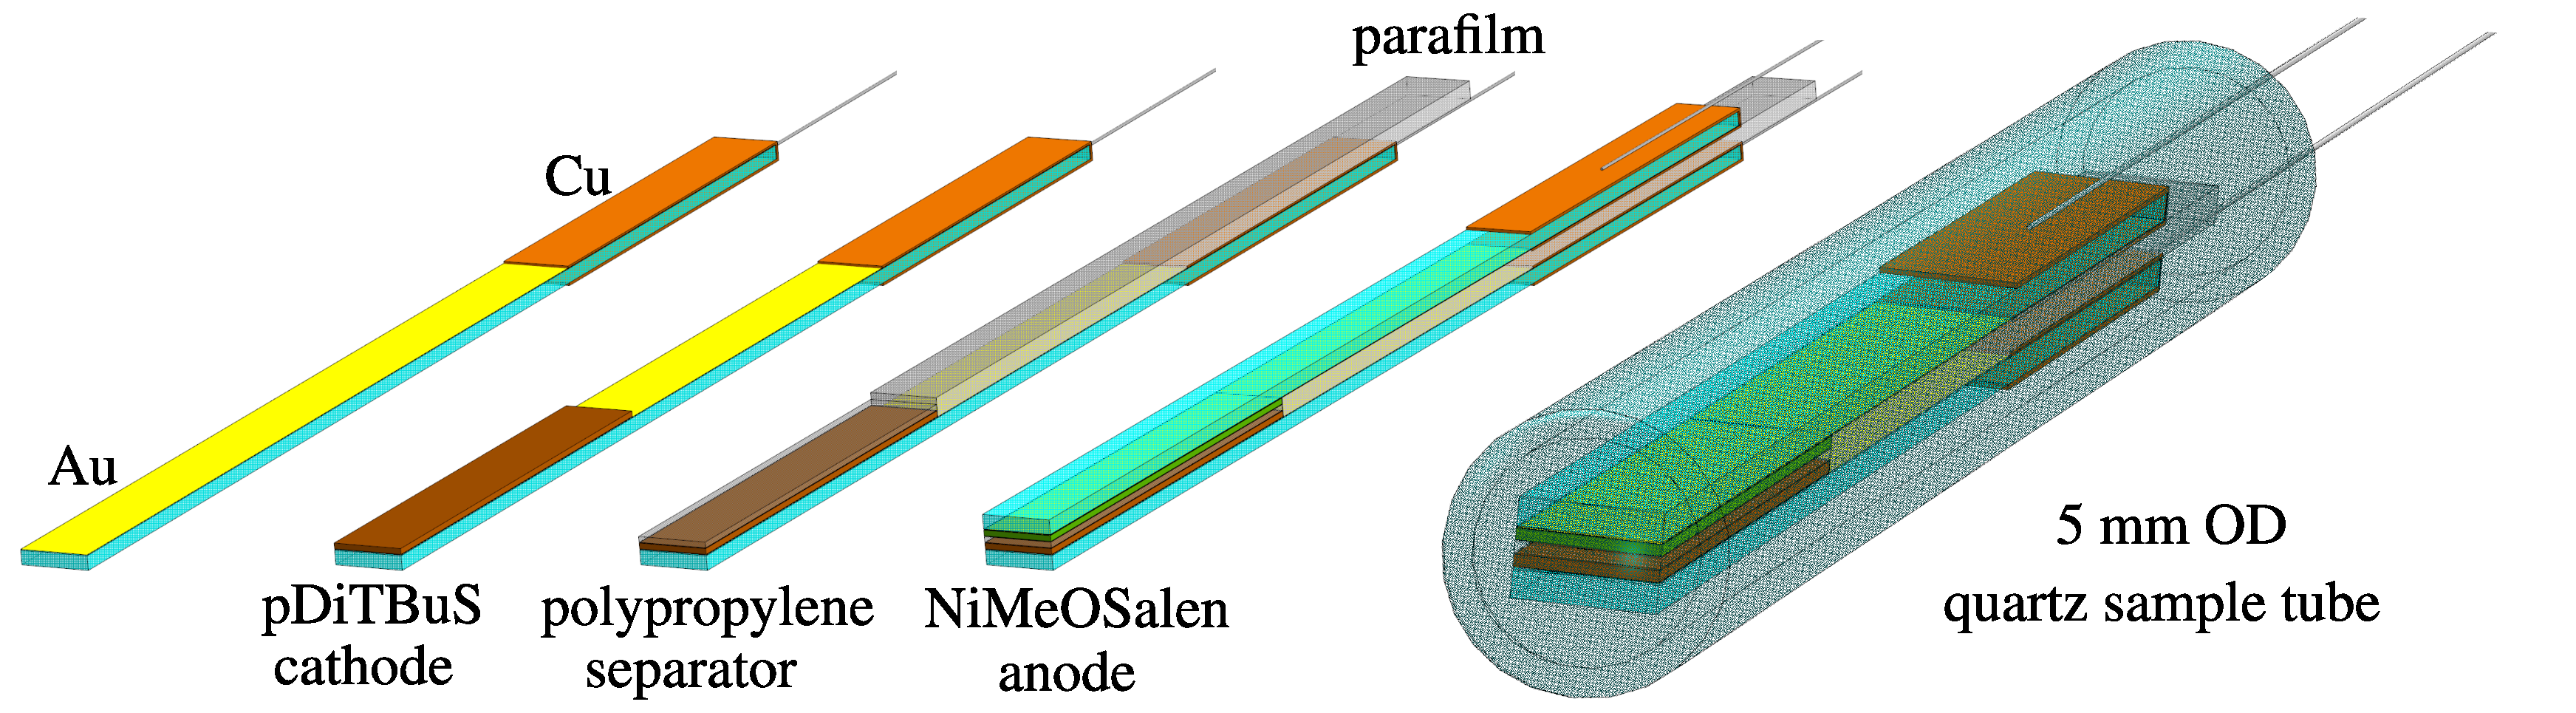
\includegraphics[width=1\textwidth]{./operando_epr/figures/sandwich/sandwich.pdf}
	\caption{All-polymer solid state organic radical battery produced between two Au-plated substrates.}
	\label{fig:sandwich_assembly}
\end{figure}



\begin{figure}[h]
\center
	
\includegraphics[width=1\textwidth]{./operando_epr/figures/solid/solid_cell.pdf}
	\caption{All-polymer solid state organic radical battery produced on a 5~$\muup$m interdigitated grid.}
	\label{fig:transistor_battery_assewmbly}
\end{figure}



\section{Ex Situ Electrochemistry}
\label{sample_fab_2}
The pDiTBuS film was brought to the desired oxidation state by galvanostatic discharging with a current of 10~$\muup$A in a three-electrode electrochemical cell in a 5~ml beaker with the electrodes and the electrolyte described above.
Each potential of the film was reached by first fully charging the cell to 700~mV and then discharging it to the desired potential (labeled points in Figure~\ref{fig:Figure_S3}). When the desired potential was \ik{reached}, the output relay of the potentiostat was opened so that no current went through the cell after charging. The substrate with the WE and the pDiTBuS film was removed from the charging cell, placed in a 5~mm OD quartz EPR tube, evacuated down to $<5\times10^{-3}$~mbar, filled with He up to a pressure of 500-600 mbar, then flame sealed with a H$_2$/O$_2$ burner.

\begin{figure}[!ht]
\center
	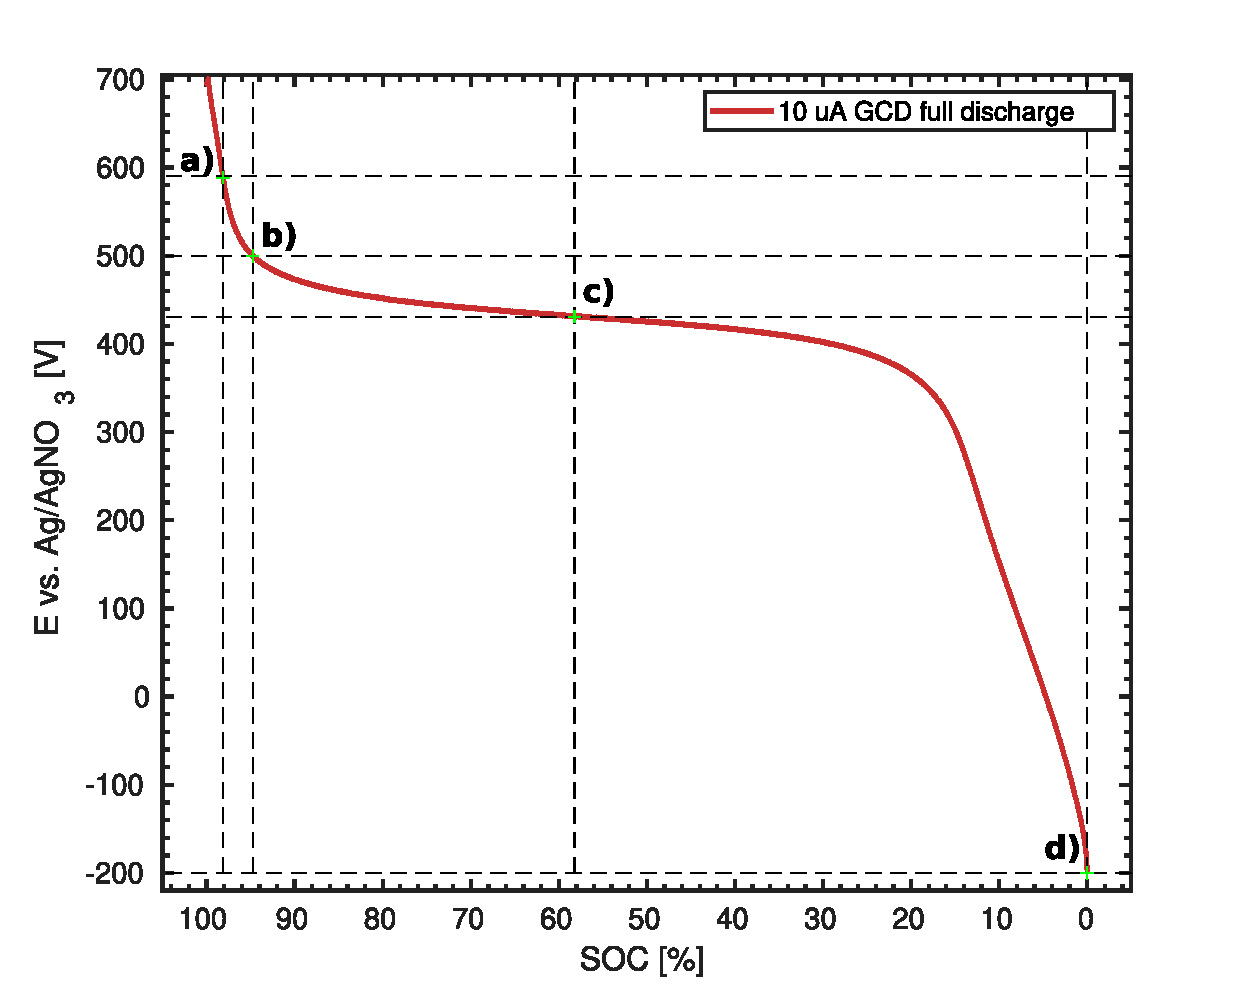
\includegraphics[width=0.85\textwidth]{./pulse/figures/Figure_S3}
	\caption{Initial galvanostatic discharge curve for the pDiTBuS film with the redox potentials described in the main text. Since the film has lost 12\% of its capacity during the temperature cycling, the SoC determined from the potentials mapped to the initial curve are lower than the SoC determined from the individual discharge curves (given in brackets). The SoC values corresponding to the initial (individual) discharge curve are a): SoC~98~(98)\%, b): SoC~\ik{94~(96)}\%, c): SoC~57(65)\%, d): SoC~0(0)\%. (Dis-)charging current: 10~$\muup$A, charging rate: 6.25~C. After this initial discharging, the pDiTBuS film has undergone 10 charge-discharge cycles and 4 temperature cycles.}
	\label{fig:Figure_S3}
\end{figure}

\begin{figure}[!ht]
\center
	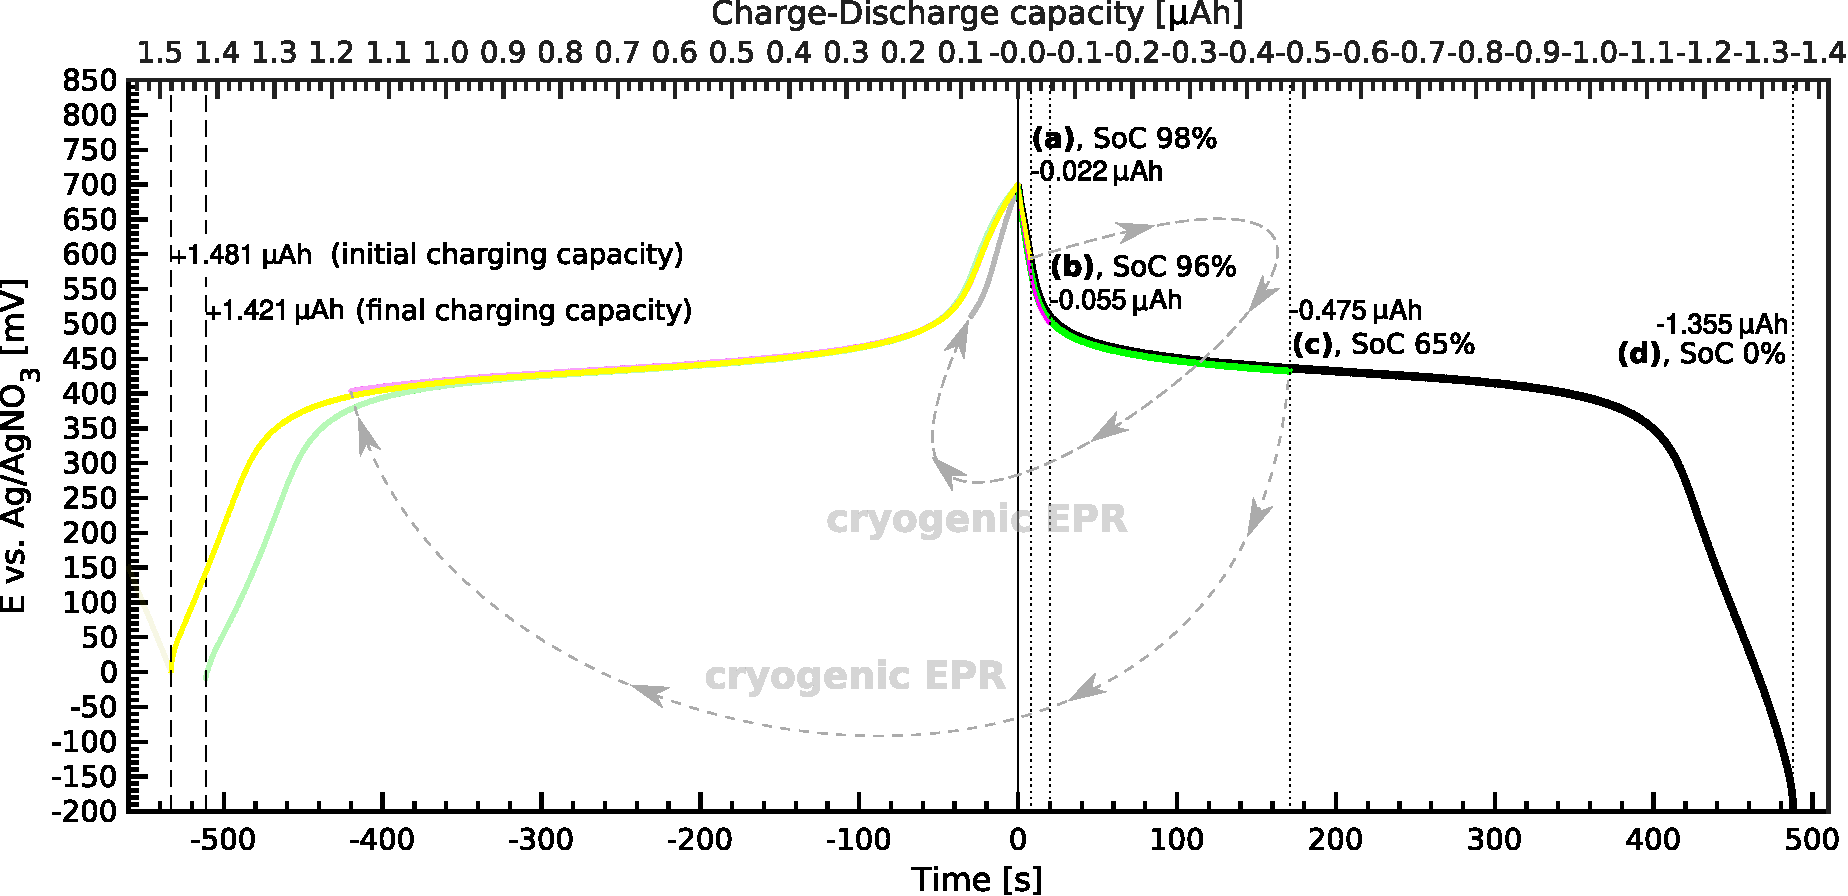
\includegraphics[width=1\textwidth]{./pulse/figures/Figure_S27}
	\caption{\ik{Calculation of the number of withdrawn electrons from a pDiTBuS film for the four states of charge. At negative times the pDiTBuS film is charged, corresponding to the withdrawal of electrons from the film. At positive times the film is discharged. The number of transferred electrons during discharging is determined from the four overlaid galvanostatic discharge curves (a-d).}}
	\label{fig:Figure_S27}
\end{figure}

\ik{
After reaching the fully charged state with 10~$\muup$A (by $t=0$ in Figure~\ref{fig:Figure_S27}), a 10~$\muup$A discharge current was applied to reach the four states of charge considered in this study (a-d in Figure~\ref{fig:Figure_S27} and in Figure~\ref{fig:Figure_S3}). Initially, the full charging capacity of the film was 1.48~$\muup$Ah~$=5.11$~\ik{m}C (3.29e+16 electrons withdrawn upon the full charging). The charging capacity has decreased by 0.06~$\muup$Ah ($4\%$) after the four temperature cycles between 300~K and 5~K during the cryogenic EPR measurements.\\
}
\newpage
\ik{
From the quantitative analysis of the GCD for each SoC, we calculate the number of elementary charges that are transferred to the film (withdrawn from the film) upon charging (discharging). The GCD and the calculated values of the transferred charge are shown in Figure~\ref{fig:Figure_S27}. During the full discharge from +700~mV down to -200~mV the pDiTBuS film has gained a total charge of 1.355~$\muup$Ah=4.88~\ik{m}C (d), corresponding to 3.01e+16 electrons that had been transferred to the film.)
}
\ik{ 
The considered SoC correspond to discharging by $0.020\pm0.005~\muup$Ah (Figure~\ref{fig:Figure_S27}~a, $(5\pm1)\times10^{14}$ electrons injected), $0.060\pm0.005~\muup$Ah (Figure~\ref{fig:Figure_S27}~b, $(1.4\pm0.1)\times10^{15}$ electrons injected), $0.480\pm0.005~\muup$Ah (Figure~\ref{fig:Figure_S27}~c, $(1.07\pm0.01)\times10^{16}$ electrons injected) and $1.360\pm0.005~\muup$Ah (Figure~\ref{fig:Figure_S27}~d, $(3.05\pm0.01)\times10^{16}$~electrons injected). The SoC values determined from the respective potentials are different when mapped to the initial discharge curve in Fig.~\ref{fig:Figure_S3} and when considering the individual discharge curves in Fig.~\ref{fig:Figure_S27}, as the film was gradually losing its capacity during the temperature cycling, so the discharge curves were reaching the considered potentials at shorter times, leading to a lower Coulomb counting, lower discharge capacity and therefore a lower SoC.}